\chapter{क्रिस्टल I: आदर्श क्रिस्टल और धातुएँ}\label{ch:b1:crystals-metals}

ताँबे के तार को बिना टूटे बाल से भी पतला खींचा जा सकता है; नमक का
डला हथौड़े की चोट से चूर-चूर हो जाता है। लोहार लोहे की छड़ को तब तक गर्म करता है
जब तक वह दहकने न लगे, उस पर हथौड़ा चलाता है, उसे पानी में डुबोता है, और छड़
पहले से कहीं अधिक कठोर होकर निकलती है। इन व्यवहारों का अंतर
ठोस में परमाणुओं के जमने के ढंग में छिपा है। अधिकांश ठोस \omterm{def:b1:crystals-metals:crystal}{क्रिस्टल} हैं:
उनके परमाणु एक ऐसे प्रतिरूप पर बैठे हैं जो हर दिशा में अरबों बार, हूबहू, अपने को
दोहराता है। यह अध्याय ऐसे प्रतिरूपों का वर्णन करता है, उनके परमाणु गिनता है,
मापता है कि वे कितनी सघनता से जमे हैं और उनके बीच के रिक्त स्थान कहाँ हैं,
और इस परिणाम से धातुओं और मिश्रधातुओं को समझता है।
अगला अध्याय यही साधन आयनिक, सहसंयोजी और आण्विक
ठोसों पर लागू करता है।

\begin{recall}
धातुएँ अपने \omterm{def:b1:quantum-numbers:configuration}{संयोजकता इलेक्ट्रॉन} आसानी से खो देती हैं: उनकी आयनन
ऊर्जाएँ और \omterm{def:b1:periodicity:electronegativity}{विद्युत-ऋणात्मकताएँ} कम होती हैं (\cref{ch:b1:periodicity})। परमाणु त्रिज्याओं
की परिभाषा \cref{def:b1:periodicity:radius} में दी गई। घनत्व, जिसका अध्ययन
भौतिकी में होता है, ज्ञात माना गया है: $\rho = m/V$।
\end{recall}

\begin{omfigure}
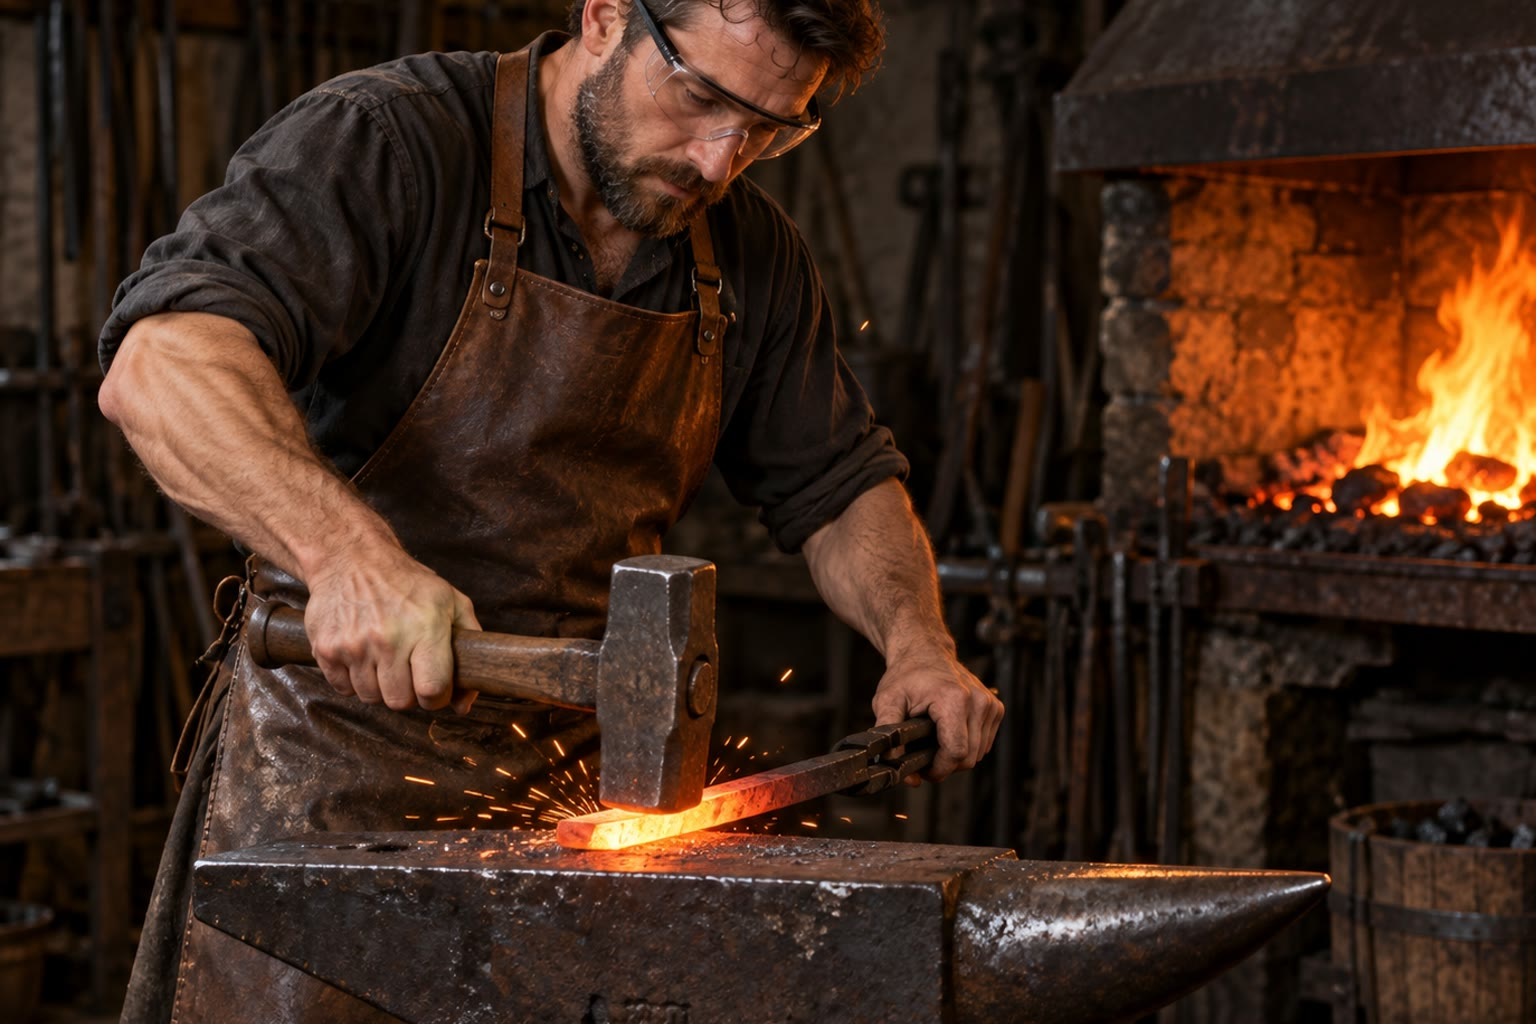
\includegraphics[width=0.55\linewidth]{images/book2/ai/b1-05-blacksmith.jpg}

{\small इस्पात गढ़ता हुआ एक लोहार। नारंगी दहकते लोहे की \omterm{def:b1:crystals-metals:crystal}{क्रिस्टल} संरचना
कमरे के ताप वाले लोहे से भिन्न होती है, और वह अधिक कार्बन धारण कर सकता है
(सप्ताहांत समस्या)।}
\end{omfigure}

\section{आदर्श-क्रिस्टल मॉडल}

\begin{definition}[क्रिस्टल, अक्रिस्टलीय ठोस, आदर्श क्रिस्टल]\label{def:b1:crystals-metals:crystal}
\emph{क्रिस्टल}\index{क्रिस्टल} वह ठोस है जिसके कण (परमाणु, आयन
या अणु) एक ऐसे प्रतिरूप में व्यवस्थित हों जो तीनों विमाओं में आवर्ती रूप से
दोहराया जाता है। ऐसी दीर्घ-परास व्यवस्था से रहित ठोस
\emph{अक्रिस्टलीय ठोस}\index{अक्रिस्टलीय ठोस} है (काँच, अधिकांश प्लास्टिक)।
\emph{आदर्श क्रिस्टल मॉडल}\index{आदर्श क्रिस्टल मॉडल} क्रिस्टल को
अनंत और दोषरहित मानता है: न कोई लुप्त या अतिरिक्त परमाणु, न कोई
अशुद्धि, न कोई सीमा।
\end{definition}

\begin{definition}[जालक, मोटिफ़, एकक कोष्ठिका]\label{def:b1:crystals-metals:lattice}
\emph{जालक}\index{जालक} बिंदुओं का एक अनंत समुच्चय है, जिनके बिंदु
\emph{जालक बिंदु}\index{जालक बिंदु} कहलाते हैं, और जो उनमें से किसी एक पर
सभी स्थानांतरण $u\,\vec a + v\,\vec b + w\,\vec c$ लगाने से मिलते हैं, जहाँ $u$, $v$,
$w$ पूर्णांक हैं। हर जालक बिंदु
पर एक ही \emph{मोटिफ़}\index{मोटिफ़} (एक परमाणु, परमाणुओं या आयनों का एक समूह)
रखने से \omterm{def:b1:crystals-metals:crystal}{क्रिस्टल} प्राप्त होता है।
\emph{एकक कोष्ठिका}\index{एकक कोष्ठिका} $\vec a$, $\vec b$, $\vec c$ पर बना एक
समांतरषट्फलक है जिसके स्थानांतरण पूरे आकाश को भर देते हैं; उसकी कोर-लंबाइयाँ
और कोण \emph{जालक प्राचल}\index{जालक प्राचल}
$a$, $b$, $c$, $\alpha$, $\beta$, $\gamma$ हैं। घनीय कोष्ठिका में
$a = b = c$ और सभी कोण $90^\circ$ होते हैं।
\end{definition}

\begin{remark}[वास्तविक क्रिस्टल]\label{rem:b1:crystals-metals:real}
वास्तविक \omterm{def:b1:crystals-metals:crystal}{क्रिस्टल} परिमित और अपूर्ण होते हैं: उनमें रिक्तियाँ,
अशुद्धियाँ, विस्थापन-रेखाएँ और कण-सीमाएँ होती हैं, जो अनेक गुणों को नियंत्रित
करती हैं (ताँबे की तन्यता, इस्पात की कठोरता)। इन
दोषों का अध्ययन तृतीय वर्ष के खंड में होता है; आदर्श \omterm{def:b1:crystals-metals:crystal}{क्रिस्टल}
ज्यामिति, घनत्व और \omterm{def:b1:crystals-metals:compactness}{संहतता} देता है, जिन्हें दोष लगभग नहीं बदलते।
\end{remark}

\begin{definition}[कोष्ठिका की बहुकता]\label{def:b1:crystals-metals:multiplicity}
किसी कोष्ठिका की \emph{बहुकता}\index{बहुकता} $Z$ उन \omterm{def:b1:crystals-metals:lattice}{मोटिफ़ों} (या परमाणुओं) की
संख्या है जो उस कोष्ठिका के हैं; पड़ोसी कोष्ठिकाओं के साथ साझा हर परमाणु
उतने भिन्न के रूप में गिना जाता है जितना उसके भीतर पड़ता है।
\end{definition}

\begin{method}[कोष्ठिका के परमाणु गिनना]\label{met:b1:crystals-metals:count}
घनीय कोष्ठिका में कोने का परमाणु 8 कोष्ठिकाओं में साझा होता है और
$1/8$ गिना जाता है; कोर पर वह 4 में साझा होता है और $1/4$ गिना जाता है; फलक पर
2 में साझा होता है और $1/2$ गिना जाता है; भीतर वह 1 गिना जाता है। योगदानों को जोड़िए।
\end{method}

\begin{definition}[उपसहसंयोजन संख्या]\label{def:b1:crystals-metals:coordination}
किसी ठोस में किसी कण की \emph{उपसहसंयोजन संख्या}\index{उपसहसंयोजन संख्या}
उसके निकटतम पड़ोसियों की संख्या है, यानी सबसे कम
दूरी पर स्थित पड़ोसियों की।
\end{definition}

\begin{definition}[संहतता]\label{def:b1:crystals-metals:compactness}
कठोर गोलों के किसी \omterm{def:b1:crystals-metals:crystal}{क्रिस्टल} की \emph{संहतता}\index{संहतता} (या संकुलन भिन्न)
आयतन का वह भिन्न है जो गोलों द्वारा घेरा गया है: आयतन $V$ वाली कोष्ठिका के लिए,
जिसमें $Z$ गोले हैं और हर गोले की त्रिज्या $R$ है,
\[
  C = \frac{Z \cdot \frac43 \pi R^3}{V} .
\]
\end{definition}

\begin{proposition}[कोष्ठिका से घनत्व]\label{prop:b1:crystals-metals:density}
जिस \omterm{def:b1:crystals-metals:crystal}{क्रिस्टल} की आयतन $V$ वाली कोष्ठिका में $Z$
कण हों, जिनका मोलर द्रव्यमान $M$ है, उसका घनत्व है
\[
  \rho = \frac{Z\,M}{N_A\,V} .
\]
\end{proposition}

\begin{proof}
कोष्ठिका में $Z$ कण हैं, जिनका द्रव्यमान $Z\,M/N_A$ है; \omterm{def:b1:crystals-metals:crystal}{क्रिस्टल}
उसी कोष्ठिका की पुनरावृत्ति है, इसलिए उसका घनत्व एक कोष्ठिका का घनत्व है।
\end{proof}

\section{निविड़ संकुलन: फलक-केंद्रित घनीय और षट्कोणीय}

\begin{definition}[निविड़ संकुलन, FCC, HCP]\label{def:b1:crystals-metals:packings}
सर्वसम गोलों का \emph{निविड़ संकुलन}\index{निविड़ संकुलन} निविड़
संकुलित परतों से बनता है, जिनमें हर गोला छह अन्य गोलों को छूता है, और जो इस तरह जमाई जाती हैं
कि किसी परत का हर गोला नीचे वाली परत के एक गड्ढे में बैठे।
जमाव $ABCABC\dots$ से \emph{फलक-केंद्रित घनीय}\index{फलक-केंद्रित घनीय}
संरचना (FCC, या घनीय निविड़ संकुलित) बनती है; जमाव $ABAB\dots$
से \emph{षट्कोणीय निविड़ संकुलित}\index{षट्कोणीय निविड़ संकुलित}
संरचना (HCP)। धातुओं की एक तीसरी, निविड़ न संकुलित, संरचना
\emph{अंतःकेंद्रित घनीय}\index{अंतःकेंद्रित घनीय} संरचना (BCC) है: एक
घन जिसके हर कोने पर एक परमाणु और केंद्र पर एक परमाणु होता है।
\end{definition}

\begin{omfigure}
\begin{tikzpicture}[font=\small]
  % layer A
  \foreach \i in {0,...,4} \foreach \j in {0,...,3} {
    \pgfmathsetmacro\x{\i+0.5*\j}
    \pgfmathsetmacro\y{0.866*\j}
    \draw[black!60, fill=omDef!25] (\x,\y) circle (0.5);
  }
  % layer B, in the hollows pointing up
  \foreach \i/\j in {1/0, 2/0, 3/0, 1/1, 2/1, 3/1, 1/2, 2/2} {
    \pgfmathsetmacro\x{\i+0.5*\j}
    \pgfmathsetmacro\y{0.866*\j+0.577}
    \draw[omThm!80!black, fill=omThm!25, fill opacity=0.75] (\x,\y) circle (0.5);
  }
  % C positions
  \foreach \i/\j in {1/0, 2/0, 3/0, 1/1, 2/1, 3/1} {
    \pgfmathsetmacro\x{\i+0.5+0.5*\j}
    \pgfmathsetmacro\y{0.866*\j+0.289}
    \fill[omMeth] (\x,\y) circle (0.11);
  }
  \node[anchor=west, align=left] at (6.6,1.6) {A: पहली परत (नीली)\\B: दूसरी परत, A के\\\phantom{B: }गड्ढों में (लाल)\\C: दूसरे गड्ढे\\\phantom{C: }(हरे बिंदु)};
\end{tikzpicture}

{\small ऊपर से देखी गई दो निविड़ संकुलित परतें। तीसरी परत C से अंकित
गड्ढों के ऊपर बैठ सकती है (जमाव $ABC$, \omterm{def:b1:crystals-metals:packings}{फलक-केंद्रित घनीय}) या
A के परमाणुओं के ऊपर (जमाव $AB$, \omterm{def:b1:crystals-metals:packings}{षट्कोणीय निविड़ संकुलित})।}
\end{omfigure}

\begin{proposition}[फलक-केंद्रित घनीय]\label{prop:b1:crystals-metals:fcc}
FCC संरचना में परमाणु कोर $a$ वाले घन के आठ कोनों और छह फलक-केंद्रों
पर होते हैं। तब $Z = 4$, \omterm{def:b1:crystals-metals:coordination}{उपसहसंयोजन संख्या}
12 है, परमाणु फलक-विकर्ण के अनुदिश एक-दूसरे को छूते हैं, $a\sqrt2 = 4R$, और
\omterm{def:b1:crystals-metals:compactness}{संहतता} है
\[
  C = \frac{\pi}{3\sqrt2} \approx 0.74 .
\]
\end{proposition}

\begin{proof}
$Z = 8 \times \frac18 + 6 \times \frac12 = 4$। फलक-केंद्र का परमाणु अपने फलक
के चार कोनों को और उस फलक को साझा करने वाली दोनों कोष्ठिकाओं में से हर एक के चार
फलक-केंद्रों को छूता है: $4 + 4 + 4 = 12$ पड़ोसी, $a\sqrt2/2$ दूरी पर। लंबाई $a\sqrt2$ वाले
फलक-विकर्ण पर एक कोने का परमाणु, एक फलक-केंद्र का परमाणु
और एक कोने का परमाणु परस्पर संपर्क में होते हैं: $a\sqrt2 = 4R$। तब
$C = 4 \cdot \frac43\pi R^3/a^3 = \frac{16}{3}\pi R^3/(2\sqrt2 R)^3 \cdot
\frac{1}{1} = \frac{16\pi}{3 \times 16\sqrt2} = \frac{\pi}{3\sqrt2}$।
\end{proof}

\begin{omfigure}
\tdplotsetmaincoords{60}{100}
\begin{tikzpicture}[tdplot_main_coords, font=\small]
  \pic {omcubeo={3}};
  \node[cellA=6mm] at (0,0,0) {};
  \node[cellA=6mm] at (0,3,0) {};
  \node[cellA=6mm, ball color=omDef!55] at (0,1.5,1.5) {};
  \node[cellA=6mm] at (0,0,3) {};
  \node[cellA=6mm, ball color=omDef!55] at (1.5,1.5,0) {};
  \node[cellA=6mm] at (0,3,3) {};
  \node[cellA=6mm, ball color=omDef!55] at (1.5,0,1.5) {};
  \node[cellA=6mm, ball color=omDef!55] at (1.5,3,1.5) {};
  \node[cellA=6mm] at (3,0,0) {};
  \node[cellA=6mm, ball color=omDef!55] at (1.5,1.5,3) {};
  \node[cellA=6mm] at (3,3,0) {};
  \node[cellA=6mm, ball color=omDef!55] at (3,1.5,1.5) {};
  \node[cellA=6mm] at (3,0,3) {};
  \node[cellA=6mm] at (3,3,3) {};
  \draw[omThm, thick] (3,0,0) -- (3,3,3);
\end{tikzpicture}
\hspace{1.2cm}
\begin{tikzpicture}[tdplot_main_coords, font=\small]
  \pic {omcubeo={3}};
  \node[cellA=7mm] at (0,0,0) {};
  \node[cellA=7mm] at (0,3,0) {};
  \node[cellA=7mm] at (0,0,3) {};
  \node[cellA=7mm] at (0,3,3) {};
  \node[cellA=7mm, ball color=omDef!55] at (1.5,1.5,1.5) {};
  \node[cellA=7mm] at (3,0,0) {};
  \node[cellA=7mm] at (3,3,0) {};
  \node[cellA=7mm] at (3,0,3) {};
  \node[cellA=7mm] at (3,3,3) {};
  \draw[omThm, thick] (3,0,0) -- (0,3,3);
\end{tikzpicture}

{\small बाएँ: \omterm{def:b1:crystals-metals:packings}{फलक-केंद्रित घनीय} कोष्ठिका (कोने के परमाणु धूसर, फलक-केंद्र के
परमाणु नीले)। परमाणु फलक-विकर्ण के अनुदिश छूते हैं (लाल रेखा,
$a\sqrt2 = 4R$)। दाएँ: \omterm{def:b1:crystals-metals:packings}{अंतःकेंद्रित घनीय} कोष्ठिका; परमाणु
मुख्य विकर्ण के अनुदिश छूते हैं (लाल रेखा, $a\sqrt3 = 4R$)।
स्पष्टता के लिए परमाणु अपने संपर्क-आकार से छोटे बनाए गए हैं।}
\end{omfigure}

\begin{proposition}[षट्कोणीय निविड़ संकुलित]\label{prop:b1:crystals-metals:hcp}
HCP संरचना में आधार-कोर $a$
और ऊँचाई $c$ वाले परंपरागत षट्कोणीय प्रिज़्म में 6 परमाणु होते हैं; \omterm{def:b1:crystals-metals:coordination}{उपसहसंयोजन संख्या} 12 है;
स्पर्श करते गोलों के लिए $a = 2R$, $c/a = \sqrt{8/3} \approx 1.633$, और
\omterm{def:b1:crystals-metals:compactness}{संहतता} FCC के समान है, $\pi/(3\sqrt2) \approx 0.74$।
\end{proposition}

\begin{proof}
प्रिज़्म के 12 कोने के परमाणु 6 प्रिज़्मों में साझा हैं, 2 फलक-केंद्र के परमाणु
2 में, और 3 परमाणु भीतर हैं: $12/6 + 2/2 + 3 = 6$। हर परमाणु अपनी परत के
छह पड़ोसियों को और हर निकटवर्ती परत के तीन पड़ोसियों को छूता है: 12। परत B का
एक परमाणु परत A के तीन परस्पर स्पर्श करते परमाणुओं पर बैठता है, और कोर $2R$ वाला
एक नियमित चतुष्फलक बनाता है, जिसकी ऊँचाई $2R\sqrt{2/3}$ है; दो परतों
की दूरी पर $c = 4R\sqrt{2/3}$, इसलिए $c/a = 2\sqrt{2/3} = \sqrt{8/3}$। प्रिज़्म का
आयतन $\frac{3\sqrt3}{2}a^2 c = \frac{3\sqrt3}{2}(2R)^2 \cdot
4R\sqrt{2/3} = 24\sqrt2\,R^3$ है, और $C = 6 \cdot \frac43\pi R^3/(24\sqrt2
R^3) = \pi/(3\sqrt2)$।
\end{proof}

\begin{omfigure}
\tdplotsetmaincoords{70}{113}
\begin{tikzpicture}[tdplot_main_coords, font=\small, scale=1.25]
  \pic[transform shape] {omhexprismo={1.6}{2.6}};
  \node[cellA=6mm] at (-1.6,0,0) {};
  \node[cellA=6mm] at (-0.8,-1.386,0) {};
  \node[cellA=6mm] at (-1.6,0,2.6) {};
  \node[cellA=6mm] at (-0.8,-1.386,2.6) {};
  \node[cellA=6mm] at (-0.8,1.386,0) {};
  \node[cellA=6mm, ball color=omThm!60] at (-0.8,0.462,1.3) {};
  \node[cellA=6mm] at (0,0,0) {};
  \node[cellA=6mm, ball color=omThm!60] at (0,-0.924,1.3) {};
  \node[cellA=6mm] at (0.8,-1.386,0) {};
  \node[cellA=6mm] at (-0.8,1.386,2.6) {};
  \node[cellA=6mm] at (0,0,2.6) {};
  \node[cellA=6mm] at (0.8,-1.386,2.6) {};
  \node[cellA=6mm] at (0.8,1.386,0) {};
  \node[cellA=6mm, ball color=omThm!60] at (0.8,0.462,1.3) {};
  \node[cellA=6mm] at (1.6,0,0) {};
  \node[cellA=6mm] at (0.8,1.386,2.6) {};
  \node[cellA=6mm] at (1.6,0,2.6) {};
\end{tikzpicture}

{\small \omterm{def:b1:crystals-metals:packings}{षट्कोणीय निविड़ संकुलित} प्रिज़्म, आधार-कोर $a$ (षट्भुज की
भुजा) और ऊँचाई $c$ वाला: परतें A (धूसर) नीचे और ऊपर,
परत B (लाल) बीच में, A के गड्ढों में बैठी हुई।}
\end{omfigure}

\section{अंतःकेंद्रित घनीय और धात्विक तत्व}

\begin{proposition}[अंतःकेंद्रित घनीय]\label{prop:b1:crystals-metals:bcc}
BCC संरचना में $Z = 2$, \omterm{def:b1:crystals-metals:coordination}{उपसहसंयोजन संख्या} 8 है, परमाणु
घन के मुख्य विकर्ण के अनुदिश छूते हैं, $a\sqrt3 = 4R$, और
\omterm{def:b1:crystals-metals:compactness}{संहतता} है
\[
  C = \frac{\pi\sqrt3}{8} \approx 0.68 .
\]
\end{proposition}

\begin{proof}
$Z = 8 \times \frac18 + 1 = 2$। केंद्रीय परमाणु आठों
कोनों को छूता है: मुख्य विकर्ण $a\sqrt3$ पर एक कोना, केंद्र और एक
कोना हैं, $a\sqrt3 = 4R$। तब $C = 2 \cdot \frac43\pi R^3/a^3 =
\frac83\pi R^3 (\sqrt3/(4R))^3 = \frac83\pi \cdot \frac{3\sqrt3}{64} =
\frac{\pi\sqrt3}{8}$।
\end{proof}

\begin{proposition}[निविड़ संकुलन सबसे सघन है]\label{prop:b1:crystals-metals:kepler}
सर्वसम गोलों के किसी भी संकुलन की \omterm{def:b1:crystals-metals:compactness}{संहतता}
$\pi/(3\sqrt2) \approx 0.7405$ से, जो FCC और HCP का मान है, अधिक नहीं होती।
\end{proposition}
\admitted

\begin{history}[केप्लर का अनुमान, 1611--2017]
हिमकणों पर 1611 में लिखे एक छोटे निबंध में योहानेस केप्लर ने कहा
कि तोप के गोलों को जमाने का कोई भी ढंग पंसारी के पिरामिड, यानी
\omterm{def:b1:crystals-metals:packings}{फलक-केंद्रित घनीय} संकुलन, से सघन नहीं हो सकता। यह कथन लगभग चार शताब्दियों तक
सिद्ध नहीं हो सका। थॉमस हेल्स ने 1998 में कंप्यूटर की सहायता से एक उपपत्ति दी,
और कंप्यूटर द्वारा पंक्ति-दर-पंक्ति जाँची गई एक औपचारिक उपपत्ति 2014 में पूरी हुई
और 2017 में प्रकाशित हुई।
\end{history}

\begin{example}[तीन धातुएँ]\label{ex:b1:crystals-metals:metals}
कॉपर FCC है, $a = \qty{361.5}{pm}$ के साथ: $R = a\sqrt2/4 =
\qty{127.8}{pm}$ और $\rho = 4 \times 63.55/(6.022 \times 10^{23} \times
(3.615 \times 10^{-8})^3) = \qty{8.93}{g/cm^3}$, जो मापा गया घनत्व है।
कमरे के ताप पर आयरन ($\alpha$-आयरन) BCC है, $a = \qty{286.7}{pm}$ के साथ:
$R = \qty{124.1}{pm}$, $\rho = \qty{7.87}{g/cm^3}$। मैग्नीशियम HCP है,
$a = \qty{320.9}{pm}$ और $c = \qty{521.0}{pm}$ के साथ: $c/a = 1.624$, जो
आदर्श $1.633$ के पास है; ज़िंक, $c/a = 1.856$ के साथ, एक लंबोतरा षट्कोणीय
संकुलन है।
% ledger: lat:Cu, rho:Cu, lat:Fe-alpha, rho:Fe, lat:Mg.a, lat:Mg.c,
% lat:Zn.a, lat:Zn.c, aw:Cu, aw:Fe, const:NA
\end{example}

\begin{center}
\small
\begin{tabular}{lllccc}
\hline
धातु & संरचना & $a$ (pm) & $R$ (pm) & $\rho$ परिकलित & $\rho$ मापित \\
\hline
ऐलुमिनियम & FCC & 405.0 & 143.2 & 2.70 & 2.70 \\
कॉपर & FCC & 361.5 & 127.8 & 8.93 & 8.93 \\
सिल्वर & FCC & 408.6 & 144.5 & 10.50 & 10.50 \\
सोडियम & BCC & 429.1 & 185.8 & 0.967 & 0.97 \\
$\alpha$-आयरन & BCC & 286.7 & 124.1 & 7.87 & 7.87 \\
टंगस्टन & BCC & 316.5 & 137.0 & 19.26 & 19.3 \\
\hline
\end{tabular}
\end{center}
% ledger: lat:Al, lat:Cu, lat:Ag, lat:Na, lat:Fe-alpha, lat:W, rho:Al,
% rho:Cu, rho:Ag, rho:Na, rho:Fe, rho:W (densities in g/cm3)

\begin{omfigure}
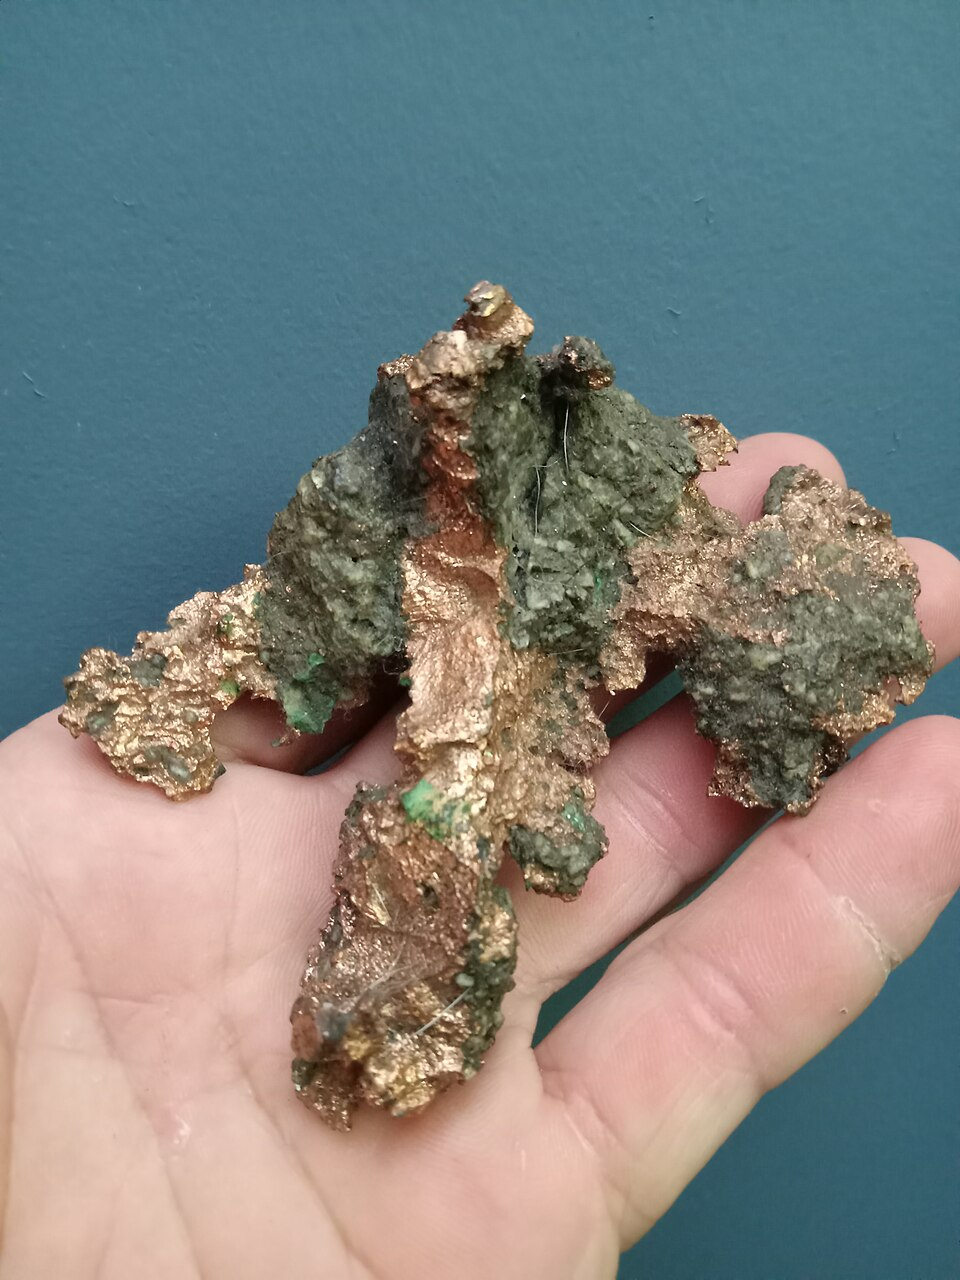
\includegraphics[width=0.36\linewidth]{images/book2/native-copper.jpg}

{\small देशी ताँबे का एक नमूना। इसकी शाखित आकृतियाँ \omterm{def:b1:crystals-metals:crystal}{क्रिस्टलों}
के रूप में बढ़ीं; नीचे की धातु FCC कणों की पच्चीकारी है।
छायाचित्र: CC0 (विकिमीडिया कॉमन्स)।}
\end{omfigure}

\section{अंतराकाशी स्थल}

\begin{definition}[अंतराकाशी स्थल]\label{def:b1:crystals-metals:site}
\emph{अंतराकाशी स्थल}\index{अंतराकाशी स्थल} किसी \omterm{def:b1:crystals-metals:crystal}{क्रिस्टल} के परमाणुओं के बीच का
ऐसा रिक्त स्थान है जहाँ कोई छोटा परमाणु बैठ सकता है। \emph{चतुष्फलकीय
स्थल}\index{चतुष्फलकीय स्थल} चार परमाणुओं के चतुष्फलक के केंद्र पर होता है,
\emph{अष्टफलकीय स्थल}\index{अष्टफलकीय स्थल} छह परमाणुओं के अष्टफलक के
केंद्र पर। किसी स्थल की \emph{आवास-क्षमता}\index{आवास-क्षमता} उस सबसे बड़े गोले
की त्रिज्या है जो आसपास के परमाणुओं को धकेले बिना उसमें
समा जाए।
\end{definition}

\begin{proposition}[FCC संरचना के स्थल]\label{prop:b1:crystals-metals:sites}
FCC कोष्ठिका में 4 \omterm{def:b1:crystals-metals:site}{अष्टफलकीय स्थल} होते हैं, घन के केंद्र पर और
उसके 12 कोरों के मध्य-बिंदुओं पर, और 8 \omterm{def:b1:crystals-metals:site}{चतुष्फलकीय स्थल}, कोर $a/2$ वाले
8 छोटे घनों के केंद्रों पर। त्रिज्या $R$ के स्पर्श करते परमाणुओं के लिए
\omterm{def:b1:crystals-metals:site}{आवास-क्षमताएँ} हैं
\[
  r_O = (\sqrt2 - 1)R \approx 0.414\,R, \qquad
  r_T = \left(\sqrt{\tfrac32} - 1\right)R \approx 0.225\,R .
\]
\end{proposition}

\begin{proof}
\omterm{def:b1:crystals-metals:site}{अष्टफलकीय स्थल}: $1 + 12 \times \frac14 = 4$, उतने ही जितने परमाणु। घन का
केंद्र छह फलक-केंद्रों से $a/2$ दूर है: $r_O + R = a/2$,
जहाँ $a = 2\sqrt2 R$, इसलिए $r_O = (\sqrt2 - 1)R$। \omterm{def:b1:crystals-metals:site}{चतुष्फलकीय स्थल}: कोर
$a/2$ वाले छोटे घन का केंद्र एकांतर कोनों पर स्थित चार परमाणुओं से
अपने मुख्य विकर्ण की आधी दूरी,
$\frac{a}{2}\cdot\frac{\sqrt3}{2} = \frac{a\sqrt3}{4}$, पर है:
$r_T + R = \frac{\sqrt3}{4}\,2\sqrt2\,R =
\sqrt{\tfrac32}\,R$।
\end{proof}

\begin{omfigure}
\tdplotsetmaincoords{60}{100}
\begin{tikzpicture}[tdplot_main_coords, font=\small]
  \pic {omcubeo={3}};
  \node[cellA=3.6mm] at (0,0,0) {};
  \node[cellsite=4mm, draw=omThm, fill=omThm!30] at (0,1.5,0) {};
  \node[cellA=3.6mm] at (0,3,0) {};
  \node[cellsite=4mm, draw=omThm, fill=omThm!30] at (0,0,1.5) {};
  \node[cellA=3.6mm] at (0,1.5,1.5) {};
  \node[cellsite=4mm, draw=omThm, fill=omThm!30] at (0,3,1.5) {};
  \node[cellsite=4mm, draw=omThm, fill=omThm!30] at (1.5,0,0) {};
  \node[cellA=3.6mm] at (0,0,3) {};
  \node[cellA=3.6mm] at (1.5,1.5,0) {};
  \node[cellsite=4mm, draw=omThm, fill=omThm!30] at (0,1.5,3) {};
  \node[cellsite=4mm, draw=omThm, fill=omThm!30] at (1.5,3,0) {};
  \node[cellA=3.6mm] at (0,3,3) {};
  \node[cellA=3.6mm] at (1.5,0,1.5) {};
  \node[cellsite=5mm, draw=omThm, fill=omThm!30] at (1.5,1.5,1.5) {};
  \node[cellA=3.6mm] at (1.5,3,1.5) {};
  \node[cellA=3.6mm] at (3,0,0) {};
  \node[cellsite=4mm, draw=omThm, fill=omThm!30] at (1.5,0,3) {};
  \node[cellsite=4mm, draw=omThm, fill=omThm!30] at (3,1.5,0) {};
  \node[cellA=3.6mm] at (1.5,1.5,3) {};
  \node[cellA=3.6mm] at (3,3,0) {};
  \node[cellsite=4mm, draw=omThm, fill=omThm!30] at (1.5,3,3) {};
  \node[cellsite=4mm, draw=omThm, fill=omThm!30] at (3,0,1.5) {};
  \node[cellA=3.6mm] at (3,1.5,1.5) {};
  \node[cellsite=4mm, draw=omThm, fill=omThm!30] at (3,3,1.5) {};
  \node[cellA=3.6mm] at (3,0,3) {};
  \node[cellsite=4mm, draw=omThm, fill=omThm!30] at (3,1.5,3) {};
  \node[cellA=3.6mm] at (3,3,3) {};
  \node[below] at (1.5,1.5,-1.5) {अष्टफलकीय स्थल (लाल)};
\end{tikzpicture}
\hspace{1.2cm}
\begin{tikzpicture}[tdplot_main_coords, font=\small]
  \pic {omcubeo={3}};
  \node[cellA=3.6mm] at (0,0,0) {};
  \node[cellA=3.6mm] at (0,3,0) {};
  \node[cellA=3.6mm] at (0,1.5,1.5) {};
  \node[cellsite=4mm, fill=omDef!30] at (0.75,0.75,0.75) {};
  \node[cellsite=4mm, fill=omDef!30] at (0.75,2.25,0.75) {};
  \node[cellA=3.6mm] at (0,0,3) {};
  \node[cellA=3.6mm] at (1.5,1.5,0) {};
  \node[cellsite=4mm, fill=omDef!30] at (0.75,0.75,2.25) {};
  \node[cellA=3.6mm] at (0,3,3) {};
  \node[cellA=3.6mm] at (1.5,0,1.5) {};
  \node[cellsite=4mm, fill=omDef!30] at (0.75,2.25,2.25) {};
  \node[cellsite=4mm, fill=omDef!30] at (2.25,0.75,0.75) {};
  \node[cellA=3.6mm] at (1.5,3,1.5) {};
  \node[cellA=3.6mm] at (3,0,0) {};
  \node[cellsite=4mm, fill=omDef!30] at (2.25,2.25,0.75) {};
  \node[cellA=3.6mm] at (1.5,1.5,3) {};
  \node[cellA=3.6mm] at (3,3,0) {};
  \node[cellsite=4mm, fill=omDef!30] at (2.25,0.75,2.25) {};
  \node[cellsite=4mm, fill=omDef!30] at (2.25,2.25,2.25) {};
  \node[cellA=3.6mm] at (3,1.5,1.5) {};
  \node[cellA=3.6mm] at (3,0,3) {};
  \node[cellA=3.6mm] at (3,3,3) {};
  \draw[omDef!70!black, thin] (0,0,0) -- (0.75,0.75,0.75) -- (1.5,1.5,0)
    (0.75,0.75,0.75) -- (1.5,0,1.5) (0.75,0.75,0.75) -- (0,1.5,1.5);
  \node[below] at (1.5,1.5,-1.5) {चतुष्फलकीय स्थल (नीले)};
\end{tikzpicture}

{\small FCC कोष्ठिका के \omterm{def:b1:crystals-metals:site}{अंतराकाशी स्थल}। बाएँ: केंद्र वाला \omterm{def:b1:crystals-metals:site}{अष्टफलकीय
स्थल} और कोरों के मध्य वाले स्थल (चार कोष्ठिकाओं में साझा)। दाएँ:
घन के आठवें भागों के केंद्रों पर आठ \omterm{def:b1:crystals-metals:site}{चतुष्फलकीय स्थल},
जिनमें से एक अपने चार परमाणुओं से जुड़ा दिखाया गया है।}
\end{omfigure}

\section{धात्विक आबंधन और मिश्रधातुएँ}

\begin{definition}[धात्विक आबंध]\label{def:b1:crystals-metals:metallic-bond}
\emph{धात्विक आबंध}\index{धात्विक आबंध} में धातु का हर परमाणु
अपने \omterm{def:b1:quantum-numbers:configuration}{संयोजकता इलेक्ट्रॉन} पूरे \omterm{def:b1:crystals-metals:crystal}{क्रिस्टल} को दे देता है: ठोस धनायनों का एक \omterm{def:b1:crystals-metals:lattice}{जालक}
है जो ऐसे इलेक्ट्रॉनों में डूबा है जो किसी विशेष परमाणु के नहीं हैं और
उसमें मुक्त रूप से गति करते हैं। आबंध धनायनों और इस साझा इलेक्ट्रॉन मेघ के बीच का
आकर्षण है; यह दिशात्मक नहीं है।
\end{definition}

\begin{proposition}[धातुओं के गुण]\label{prop:b1:crystals-metals:properties}
\omterm{def:b1:crystals-metals:metallic-bond}{धात्विक आबंध} धातुओं के गुणों की व्याख्या करता है: गतिशील इलेक्ट्रॉन
विद्युत और ऊष्मा का चालन करते हैं और प्रकाश को परावर्तित करते हैं (चमक); चूँकि आबंध
दिशात्मक नहीं है, परमाणुओं की परतें \omterm{def:b1:crystals-metals:crystal}{क्रिस्टल} को तोड़े बिना एक-दूसरे पर
फिसल सकती हैं (तन्यता, आघातवर्धनीयता), और \omterm{def:b1:crystals-metals:packings}{निविड़ संकुलन}, जो
पड़ोसियों की संख्या अधिकतम करते हैं, सबसे सामान्य संरचनाएँ हैं।
\end{proposition}
\admitted

\begin{definition}[मिश्रधातुएँ]\label{def:b1:crystals-metals:alloy}
मिश्रधातु कई तत्वों से बना एक धात्विक ठोस है।
\emph{प्रतिस्थापनी मिश्रधातु}\index{प्रतिस्थापनी मिश्रधातु} में मिलाए गए तत्व के
परमाणु आतिथेय के \omterm{def:b1:crystals-metals:lattice}{जालक} पर उसके परमाणुओं का स्थान लेते हैं; इसके लिए
त्रिज्याओं का एक-दूसरे से लगभग 15\,\% के भीतर होना आवश्यक है (कॉपर और निकेल, पीतल में कॉपर और
ज़िंक)। \emph{अंतराकाशी मिश्रधातु}\index{अंतराकाशी मिश्रधातु} में
छोटे परमाणु (\ce{H}, \ce{C}, \ce{N}, \ce{B}) आतिथेय के \omterm{def:b1:crystals-metals:site}{अंतराकाशी स्थलों} पर
बैठते हैं (इस्पात में कार्बन)।
\end{definition}

\begin{definition}[अपररूपता]\label{def:b1:crystals-metals:allotropy}
एक ही तत्व की विभिन्न \omterm{def:b1:crystals-metals:crystal}{क्रिस्टल} संरचनाएँ उसके
\emph{अपररूप}\index{अपररूप} हैं। आयरन कमरे के ताप पर BCC ($\alpha$-आयरन)
होता है; \qty{1189}{K} से \qty{1661}{K} तक उसे FCC ($\gamma$-आयरन) मापा गया है,
और \qty{1662}{K} पर फिर BCC ($\delta$-आयरन), जो उसके
गलनांक तक रहता है। कार्बन हीरे और ग्रेफ़ाइट के रूप में पाया जाता है
(\cref{ch:b1:crystals-ionic-covalent})।
% ledger: lat:Fe-alpha, lat:Fe-gamma-1189, lat:Fe-gamma-1661,
% lat:Fe-delta-1662
\end{definition}

\begin{example}[इस्पात]\label{ex:b1:crystals-metals:steel}
कार्बन, जिसकी \omterm{def:b1:periodicity:radius}{सहसंयोजी त्रिज्या} \qty{77}{pm} है (हीरे में \ce{C-C} दूरी की
आधी), आयरन के स्थलों के लिए बिना विकृति के बहुत बड़ा है, पर
$\gamma$-आयरन में यह समस्या कहीं कम है, जिसके \omterm{def:b1:crystals-metals:site}{अष्टफलकीय स्थल} सबसे बड़े हैं। इस्पात
गर्म $\gamma$-आयरन में कार्बन घोलकर बनाया जाता है; शमन करने पर, जब आयरन
वापस अंतःकेंद्रित संरचना में लौटता है तो कार्बन उसमें फँस जाता है, संरचना को
विकृत कर देता है, और विकृत \omterm{def:b1:crystals-metals:crystal}{क्रिस्टल} कठोर होता है।
% ledger: lat:C-diamond (r = a sqrt3 / 8 = 77.2 pm)
\end{example}

\begin{remark}[आयरन के संक्रमण]\label{rem:b1:crystals-metals:iron-T}
\cref{def:b1:crystals-metals:allotropy} के ताप वायुमंडलीय दाब पर
शुद्ध आयरन के हैं; घुला हुआ कार्बन उस ताप को घटा देता है
जिस पर $\gamma$-आयरन बनता है, और इससे इस्पात पर काम करना संभव होता है।
मिश्रधातुओं के प्रावस्था आरेखों का अध्ययन द्वितीय वर्ष के खंड में होता है।
\end{remark}

\section{अभ्यास}

\begin{exercise}[$\star$]\label{exo:b1:crystals-metals:1}
सरल घनीय कोष्ठिका (केवल कोनों पर परमाणु), BCC
कोष्ठिका और FCC कोष्ठिका के परमाणु गिनिए, और हर एक में \omterm{def:b1:crystals-metals:coordination}{उपसहसंयोजन संख्या} बताइए।
\end{exercise}

\begin{exercise}[$\star$]\label{exo:b1:crystals-metals:2}
दिखाइए कि सरल घनीय संरचना की \omterm{def:b1:crystals-metals:compactness}{संहतता} (परमाणु कोर के अनुदिश
स्पर्श करते हुए) $\pi/6$ है, और FCC तथा BCC से तुलना कीजिए।
\end{exercise}

\begin{exercise}[$\star$]\label{exo:b1:crystals-metals:3}
ऐलुमिनियम FCC है, $a = \qty{405.0}{pm}$ के साथ। उसकी परमाणु त्रिज्या और
उसका घनत्व ($M = \qty{26.98}{g/mol}$) परिकलित कीजिए।
% ledger: lat:Al, aw:Al
\end{exercise}

\begin{exercise}[$\star$]\label{exo:b1:crystals-metals:4}
सोडियम BCC है, $a = \qty{429.1}{pm}$ के साथ। उसकी परमाणु त्रिज्या और
उसका घनत्व ($M = \qty{22.99}{g/mol}$) परिकलित कीजिए, और मापे गए
\qty{0.97}{g/cm^3} से तुलना कीजिए।
% ledger: lat:Na, rho:Na, aw:Na
\end{exercise}

\begin{exercise}[$\star\star$]\label{exo:b1:crystals-metals:5}
सिल्वर FCC है और उसका घनत्व \qty{10.50}{g/cm^3} है
($M = \qty{107.87}{g/mol}$)। \omterm{def:b1:crystals-metals:lattice}{जालक प्राचल} और परमाणु
त्रिज्या परिकलित कीजिए।
% ledger: rho:Ag, aw:Ag
\end{exercise}

\begin{exercise}[$\star\star$]\label{exo:b1:crystals-metals:6}
दिखाइए कि स्पर्श करते गोलों की HCP संरचना में $c/a = \sqrt{8/3}$।
मैग्नीशियम के लिए $a = \qty{320.9}{pm}$, $c = \qty{521.0}{pm}$। $c/a$
और मैग्नीशियम का घनत्व ($M = \qty{24.31}{g/mol}$) परिकलित कीजिए।
% ledger: lat:Mg.a, lat:Mg.c, aw:Mg
\end{exercise}

\begin{exercise}[$\star\star$]\label{exo:b1:crystals-metals:7}
कोर $a$ वाली FCC कोष्ठिका में, कोष्ठिका के 4 परमाणुओं, 4 \omterm{def:b1:crystals-metals:site}{अष्टफलकीय स्थलों} और
8 \omterm{def:b1:crystals-metals:site}{चतुष्फलकीय स्थलों} के निर्देशांक बताइए। प्रति परमाणु हर प्रकार के कितने हैं?
\end{exercise}

\begin{exercise}[$\star\star$]\label{exo:b1:crystals-metals:8}
कॉपर और निकेल दोनों FCC हैं, क्रमशः $a = \qty{361.5}{pm}$ और
$a = \qty{352.4}{pm}$ के साथ। उनकी परमाणु त्रिज्याएँ परिकलित कीजिए। वे सभी अनुपातों में
\omterm{def:b1:crystals-metals:alloy}{प्रतिस्थापनी मिश्रधातु} बनाते हैं: समझाइए। हाइड्रोजन, एक बहुत छोटा परमाणु, किसी धातु के
साथ किस प्रकार की मिश्रधातु बना सकता है?
% ledger: lat:Cu, lat:Ni
\end{exercise}

\begin{exercise}[$\star\star$]\label{exo:b1:crystals-metals:9}
टंगस्टन BCC है, $a = \qty{316.5}{pm}$ के साथ। उसकी त्रिज्या, उसका
घनत्व ($M = \qty{183.84}{g/mol}$) और \qty{1}{cm^3} में परमाणुओं की
संख्या परिकलित कीजिए।
% ledger: lat:W, aw:W
\end{exercise}

\begin{exercise}[$\star\star\star$]\label{exo:b1:crystals-metals:10}
BCC संरचना में एक \omterm{def:b1:crystals-metals:site}{अष्टफलकीय स्थल} हर फलक के केंद्र पर होता है
(और हर कोर के मध्य में), और एक \omterm{def:b1:crystals-metals:site}{चतुष्फलकीय स्थल} हर फलक पर
$(\frac{a}{2}, \frac{a}{4}, 0)$ पर। दिखाइए कि उनकी
\omterm{def:b1:crystals-metals:site}{आवास-क्षमताएँ} $r_O = \frac{2 - \sqrt3}{4}\,a$ और
$r_T = \frac{\sqrt5 - \sqrt3}{4}\,a$ हैं, और इन्हें $R$ के भिन्नों के रूप में
व्यक्त कीजिए। कौन-सा स्थल बड़ा है?
\end{exercise}

\begin{exercise}[$\star\star\star$]\label{exo:b1:crystals-metals:11}
कोई धातु प्रति घनीय कोष्ठिका $Z$ परमाणुओं के साथ क्रिस्टलित होती है, और कोष्ठिका का कोर $a$ है।
दिखाइए कि
\omterm{def:b1:crystals-metals:compactness}{संहतता} को $C = \frac{4\pi R^3 Z}{3a^3}$ लिखा जा सकता है, फिर यह कि
$C = \frac{\pi\rho N_A}{6M}\,(2R)^3$। इसे कॉपर ($R = \qty{127.8}{pm}$,
$\rho = \qty{8.93}{g/cm^3}$) पर लागू करके मान $0.74$ की जाँच कीजिए।
\end{exercise}

\begin{exercise}[$\star\star\star$]\label{exo:b1:crystals-metals:12}
गोल्ड FCC है, $a = \qty{407.8}{pm}$ के साथ, और सिल्वर FCC है,
$a = \qty{408.6}{pm}$ के साथ। गोल्ड और सिल्वर सभी अनुपातों में मिलते हैं। हर एक के
50\,\% परमाणुओं वाली मिश्रधातु के \omterm{def:b1:crystals-metals:lattice}{जालक प्राचल} (औसत मान लीजिए) और उसके घनत्व
($M(\ce{Au}) = \qty{196.97}{g/mol}$,
$M(\ce{Ag}) = \qty{107.87}{g/mol}$) का अनुमान लगाइए।
% ledger: lat:Au, lat:Ag, aw:Au, aw:Ag
\end{exercise}

\section{समस्या: इस्पात कार्बन को क्यों थामता है}

\begin{problem}[{सप्ताहांत समस्या --- लगभग 1190\,K के अपने संक्रमण के नीचे और ऊपर
आयरन, उसके परमाणुओं के बीच के रिक्त स्थान, और कार्बन के लिए उनमें बची
जगह}]
\label{pb:b1:crystals-metals:1}
आँकड़े: $M(\ce{Fe}) = \qty{55.845}{g/mol}$, $M(\ce{C}) = \qty{12.011}{g/mol}$,
$N_A = \qty{6.022e23}{mol^{-1}}$। कमरे के ताप पर $\alpha$-आयरन BCC है,
$a = \qty{286.65}{pm}$ के साथ। संक्रमण के ठीक ऊपर, \qty{1189}{K} पर,
$\alpha$-आयरन (जो संक्रमण के नीचे अब भी उपस्थित है) का मापा गया मान
$a = \qty{289.8}{pm}$ है और FCC $\gamma$-आयरन का $a = \qty{363.9}{pm}$।
हीरा घनीय है, $a = \qty{356.68}{pm}$ के साथ, और हर कार्बन मुख्य विकर्ण के एक-चौथाई
पर स्थित चार अन्य कार्बनों को छूता है।
% ledger: lat:Fe-alpha, lat:Fe-alpha-1189, lat:Fe-gamma-1189,
% lat:C-diamond, aw:Fe, aw:C, const:NA

\medskip
\noindent\textbf{भाग I --- कमरे के ताप पर $\alpha$-आयरन।}
\begin{enumerate}
  \item BCC कोष्ठिका के कितने परमाणु होते हैं? \omterm{def:b1:crystals-metals:coordination}{उपसहसंयोजन
        संख्या} क्या है?
  \item परमाणु किस रेखा के अनुदिश छूते हैं? आयरन परमाणु की त्रिज्या
        परिकलित कीजिए।
  \item $\alpha$-आयरन का घनत्व परिकलित कीजिए।
  \item \qty{1}{cm^3} $\alpha$-आयरन में आयरन के कितने परमाणु हैं?
  \item BCC संरचना की \omterm{def:b1:crystals-metals:compactness}{संहतता} परिकलित कीजिए।
  \item मापे गए घनत्व, \qty{7.87}{g/cm^3}, से तुलना कीजिए।
% ledger: rho:Fe
\end{enumerate}

\medskip
\noindent\textbf{भाग II --- संक्रमण पार करना।}
\begin{enumerate}[resume]
  \item \qty{1189}{K} पर $\alpha$-आयरन में और
        $\gamma$-आयरन में आयरन परमाणु की त्रिज्या परिकलित कीजिए।
  \item हर प्रावस्था में प्रति परमाणु आयतन परिकलित कीजिए।
  \item कौन-सी प्रावस्था अधिक घनी है? दोनों घनत्व परिकलित कीजिए।
  \item गर्म करने पर जब कोई छड़ $\alpha$ से $\gamma$ में जाती है तो उसका आयतन
        कितने प्रतिशत बदलता है?
  \item क्या परिणाम दोनों संरचनाओं की \omterm{def:b1:crystals-metals:compactness}{संहतताओं} के
        अनुरूप है?
\end{enumerate}

\medskip
\noindent\textbf{भाग III --- $\alpha$-आयरन में रिक्त स्थान।}
\begin{enumerate}[resume]
  \item हीरे की संरचना से कार्बन की \omterm{def:b1:periodicity:radius}{सहसंयोजी त्रिज्या} परिकलित कीजिए।
  \item \qty{1189}{K} पर BCC $\alpha$-आयरन में एक \omterm{def:b1:crystals-metals:site}{अष्टफलकीय स्थल} की \omterm{def:b1:crystals-metals:site}{आवास-क्षमता},
        $r_O = \frac{2 - \sqrt3}{4}\,a$, परिकलित कीजिए।
  \item एक \omterm{def:b1:crystals-metals:site}{चतुष्फलकीय स्थल} की \omterm{def:b1:crystals-metals:site}{आवास-क्षमता}, $r_T = \frac{\sqrt5 -
        \sqrt3}{4}\,a$, परिकलित कीजिए।
  \item कार्बन की त्रिज्या से तुलना कीजिए। किसी कार्बन परमाणु के चारों ओर
        \omterm{def:b1:crystals-metals:lattice}{जालक} के साथ क्या होना चाहिए?
  \item समझाइए कि कार्बन $\alpha$-आयरन में केवल नगण्य मात्रा में
        क्यों घुलता है।
\end{enumerate}

\medskip
\noindent\textbf{भाग IV --- $\gamma$-आयरन में रिक्त स्थान।}
\begin{enumerate}[resume]
  \item $\gamma$-आयरन की FCC कोष्ठिका में प्रति आयरन परमाणु कितने \omterm{def:b1:crystals-metals:site}{अष्टफलकीय स्थल}
        होते हैं?
  \item $\gamma$-आयरन के एक \omterm{def:b1:crystals-metals:site}{चतुष्फलकीय स्थल} की \omterm{def:b1:crystals-metals:site}{आवास-क्षमता} परिकलित कीजिए।
  \item यदि सभी \omterm{def:b1:crystals-metals:site}{अष्टफलकीय स्थल} कार्बन से भर जाते, तो ठोस का सूत्र
        और कार्बन का द्रव्यमान अंश क्या होता?
  \item यदि दस में से एक \omterm{def:b1:crystals-metals:site}{अष्टफलकीय स्थल} भरा होता, तो कार्बन का द्रव्यमान
        अंश क्या होता?
  \item समझाइए कि इस्पात गर्म आयरन में कार्बन घोलकर क्यों बनाया जाता है।
  \item $\gamma$-आयरन के \omterm{def:b1:crystals-metals:site}{अष्टफलकीय स्थल} में समा सकने वाले सबसे बड़े गोले की
        त्रिज्या परिकलित कीजिए।
\end{enumerate}
\end{problem}
